\documentclass[12pt, a4paper]{article}
% \usepackage{mathtools}
\usepackage{graphicx}
\usepackage{amsthm}
\usepackage{hyperref}
\usepackage{amssymb}
\graphicspath{{images/}}

\hypersetup{
    colorlinks=true,
    linkcolor=blue,
    urlcolor=cyan
}

\title{AP Stats Notes}
\author{Franklin Chen}
\date{11 November 2024 - idk some time in may}

\theoremstyle{definition}
\newtheorem{definition}{Definition}

\begin{document}
\maketitle
\newpage
% comment

using \textit{The Practice of Statistics for the AP Exam: 6th Edition} by Starnes and Tabor

\section{Data Analysis}
\subsection{What is Statistics?}

\begin{definition}[Statistics]
    The science of collecting, analyzing, and drawing conclusions from data.
\end{definition}

Data is collected from \emph{individuals} about certain \emph{variables}.

\begin{definition}[Individual, Variable]
    
    \textbf{Individuals} are objects described in a dataset. Typically people, but not always.
    
    \textbf{Variables} are attributes that can take different values for different individuals.
\end{definition}

For example, \emph{individuals} may be households, and \emph{variables} may be region, nnumber of people, household income, etc. It's important to distinguish between \emph{categorial} and \emph{quantative} variables:

\begin{definition}[Categorical and Quantative Variables]
    \textbf{Categorical Variables} are variables whose values can be placed into distinct categories.

    \textbf{Quantative Variables} are variables whose values are quantities, typically counts or measurements.
\end{definition}

For example, region would be categorical, while household income would be quantative. \emph{Not all numbers are quantative}; eg. zip code.

\subsection{Analyzing Categorical Data}
\subsubsection{One-Variable Categorical Data}
\begin{definition}[Frequency and Relative Frequency Tables]
    \textbf{Frequency Tables}shows the number of individuals that have values of a certain category. \textbf{Relative Frequency Tables} shows the proportion or percent of individuals in each category.
\end{definition}

\emph{Note (relative) frequencies are not data; they \emph{summarize} data.} Bar graphs and Pie Graphs summarize relative frequency tables.

\emph{Beware of misleading graphs}; we mainly react to the area of each bar, not the actual height.

\subsubsection{Two-Variable Categorical Data}
Use a two-way table to summarize data about two categorical variables. These tables can be used to answer questions about \emph{marginal, joint, and conditional relative frequencies.}
\begin{figure}[t]
    \centering
    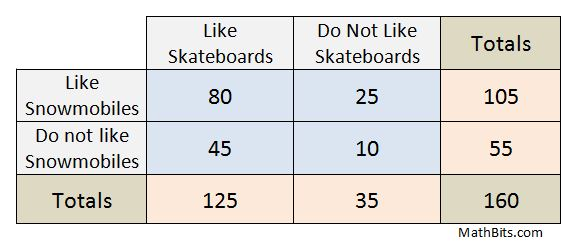
\includegraphics[width=0.75\textwidth]{two way table.png}
    \caption{An example two-way table with additional summary information.}
    \label{fig:two-way-table}
\end{figure}

\textbf{Margial relative frequencies} give the percent or proportion of individuals that have a given value for one categorical variable. For example, the marginal relative frequency of liking skateboards is $\frac{125}{160} \approx 78.125\%$.

\textbf{Joint relative frequencies} give the percent or proportion of individuals that have a specific value for both categorical variables. For example, the joint frequency of liking both skateboards and snowmobiles is $\frac{80}{160} = 50\%$.

\textbf{Conditional relative frequencies} give the percent or proportion of individuals that have a specific value for one categorical variable relative to other individuals with the same other categorical variable. For example, the conditional relative frequency of those who like snowmobiles out of all individuals that like skateboards is $\frac{80}{125} = 64\%$.

These frequencies can be summarized in \emph{side by side bar graphs, segemented bar graphs, or mosaic plots.}

Graphs and these tables can be used to show \textbf{assocation} between two variables. There is association between two variables if knowing the value of one helps to predict the other. For example, knowing that an individual likes skateboards helps predict whether they like snowmobiles ($\frac{80}{125} = 64\%$ vs $\frac{25}{35} \approx 71.4\%$). \textbf{ASSOCIATION DOES NOT IMPLY CAUSATION!}

\newpage

\subsection{Analyzing Quantative Data with Graphs}
\begin{figure}[t]
    \centering
    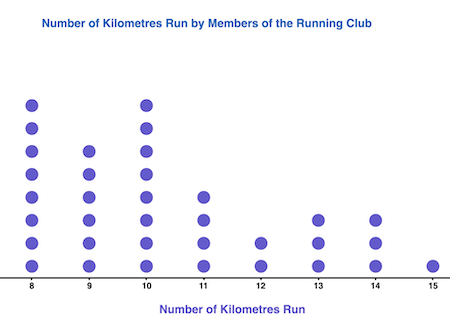
\includegraphics[width=0.75\textwidth]{dotplot.png}
    \caption{A dotplot showing the distribution of kilometers run by members of the running club.}
    \label{fig:dotplot}
\end{figure}

\emph{Dotplots} (as shown above) show each individual as a dot above their quantative data value.

When describing the shape of a dotplot (or other quantative graphs), \emph{focus on main features}: major peaks, clusters, or gaps. Especially note whether the distribution is roughly symmetric or skewed:

\begin{definition}[Symmetric, Skewed]
    A distribution is rougly \textbf{symmetric} if the right side of the graph has rougly the same shape as the left side.
    
    A distribution is \textbf{skewed to the right} if the right 'tail' has less values than the left; typically, the left has a peak whereas the right does not.
    \textbf{Left-skewed} definition are defined similarly to right-skewed distributions.
\end{definition}

For example, the distribution of the number of kilometers run is right-skewed because the right 'tail' has less values.

Graphs with a single peak are considered \emph{unimodal}, like the dotplot. Distributions with two peaks are considered \emph{bimodal}, and beyond that is considered \emph{multimodal.}

When describing a distribution of quantative data, use the acronym ROCS: \textbf{R}ange (max - min), \textbf{O}utliers (clear departures from the data), \textbf{C}enter (mean or median), and \textbf{S}hape (symmetry, skew, gaps, peaks).

Leaf plots exist. Stem represents first few digits, leaf represents final digit.

\begin{figure}[t]
    \centering
    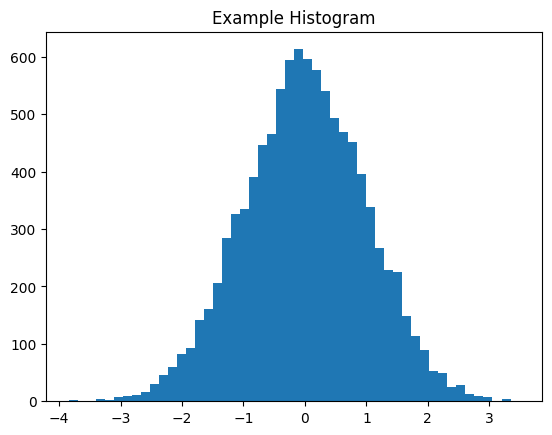
\includegraphics[width=0.75\textwidth]{histogram.png}
    \caption{An example histogram with a normal distribution.}
    \label{fig:histogram}
\end{figure}

\textbf{Histograms} are a notable way of displaying quantative data, as they avoid showing individual data points.
Histograms divide the variable into many 'bins' (bars), with the height representing the frequency. Smaller bins show more detail at the cost of a less clear pattern.

\textbf{Don't confuse histograms and bar graphs.} Histograms are used for quantative data, while bar graphs are used for qualatative data.

\textbf{Use percentages when comapring to distributions} in order to remove the effect of a larger sample.

\newpage

\subsection{Describing Quantative Data with Numbers}

\end{document}